%\textbf{TO BE COMPLETED}\\
\vspace{0.5cm}
%%\textbf{TO BE COMPLETED}\\
\vspace{0.5cm}
%%\textbf{TO BE COMPLETED}\\
\vspace{0.5cm}
%%\textbf{TO BE COMPLETED}\\
\vspace{0.5cm}
%\input{HowToAddRules}
There are three ways to add a new rule to the Modelbase: 1) add a rule to a list of common monetary policy rules, 2) include the model-specific rule calibrated or estimated by the original model authors and 3) specify a rule using the Modelbase user-specified rule option. Below we discuss each case in detail. Keep in mind that policy rules in the Modelbase have to be reformulated in terms of common Modelbase variables such as the annualized quarterly interest rate, the annualized quarter-to-quarter rate of inflation, the quarterly output and the quarterly output gap. This is explained in detail in \cite{WCMSW2012} and in the separate document, called 'MMB\_MPrule\_description.pdf'. 
%Also, one can see how it practically works by looking at common monetary policy rules already implemented in the \emph{MMB\_OPTIONS/MMB\_settings.m} file.
\newline


        \begin{figure}
        \centering
        \caption{\textsc{Taylor (1993) rule as defined in json-file}}
        \vspace{0.2cm}
        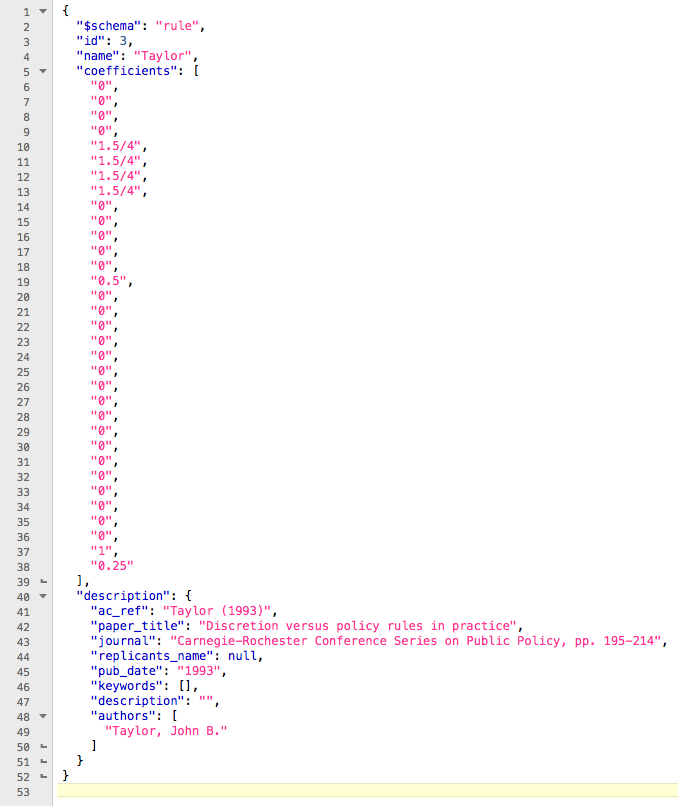
\includegraphics[width=13cm,keepaspectratio]{userrulejson.png}
        \label{img:userruletaylorjson}
        \end{figure}




\noindent {\it 1) Add a common monetary policy rule}\\
%\textbf{TO BE COMPLETED}
\begin{itemize}
%  \item The first task is to choose a suitable name for the new policy rule and to include it into an array for a list of rule names, \emph{rulenames}. One also has to add its acronyms in character arrays, \emph{rulenamesshort} and \emph{rulenamesshort1} \footnote{ As \emph{rulenamesshort1} are used for displaying simulation outcomes in Matlab console, any blank is not allowed in the rule name.}. Please make sure that the new rule name is of the same size of character array as the already existing one. Next, one assigns color to the rule with the array \textit{myrulecolor}.
%	\item Then, one adds the specification of the new-rule coefficients right after the last common rule's specification.
%  \item The remaining work is to add the new rule to the frontend of the MMB 3.0 \\\textbf{TO BE COMPLETED}.
\item In the new version of the MMB, policy rules are entirely defined via json-files. Common policy rules are stored in the subfolder `resources/app/dist/electron/static/mmci-cli/rules'.
\item The first task is to choose a suitable name for the new policy rule and to create a json-file with the same name. This json-file is to be stored in a subfolder with the exactly same name in the \textit{RULE} folder.
\item The json-file for a rule is in general similar to those for models; the whole entry has to be in curly brackets (\{...\}) and blocks are separated by commas. Figure \ref{img:userruletaylorjson} shows an exemplary json-file for the Taylor (1993) rule.
\item First, you have to indicate that the json-file describes a policy rule by setting \texttt{"\$schema": "rule"},
\item Second, you have to give the new rule an id-number by specifying \texttt{"id":\textit{number}}. The number 3 to 11 are already taken by the common policy rules shipped with the MMB.
\item Third, give your rule a name by specifying \texttt{"name": \textit{name}}, which should be the same you have given to the folder and the json-file.
\item Fourth, you have to actually specify the parameters of the rule by setting \texttt{"coefficients": $[$...$]$} to the respective values.
\item Fifth, you need to add a description of the rule, very much like you do in the json-files for models as described in section \ref{sec:ModelfileStructure}. Here, you can set \texttt{"replicants\_name": null}.
\item Safe the json-file and go to the MMB interface, click on `Menu' and `Reload Data'. The new rule should now be displayed under `Policy rules'
\item However, in order to use the new rule for comparison exercises, you also need to add its \texttt{id} to the \texttt{rules} section of all model-jsons for which the rule can/shall be used. This is necessary because not all models can be solved with all parameterizations (see subsection 3 of this chapter) and the new MMB is designed such that only common policy rules can be selected in combination with models in which they actually work. When you have done this, again reload data in the interface. The new rule should now be fully implemented in your MMB.


\end{itemize}


\noindent {\it 2) Add the model-specific monetary policy rule}

\begin{itemize}
  \item When adding a new model, it is possible to include its policy rule as long as the rule can be rewritten in terms of Modelbase common variables. If this is the case, the user should specify the parameters of the model-specific rule in the \texttt{"msr"} section of the model's json-file.
%  add the model identification number to the variable vector \emph{model\_with\_rule} in the  file \emph{MMB\_settings.m} such that a model-specific rule is activated when its corresponding model is chosen in \textbf{Option 2}. Otherwise, the user should add the model number to the variable vector \emph{model\_without\_rule}. For example, if the policy rule is set for the interest rate to react to exchange rate or credit growth, the user cannot include the original rule in the Modelbase.
%  \item Finally, the user has to insert the specification of the model-specific rule into the part of \emph{switch} statement in the file \emph{MMB\_OPTIONS/MSR\_COEFFFS.m} using the model's identification number as the case expression.
\item Reload data in the interface to employ the changes in the MMB.
\end{itemize}

\noindent {\it 3) User-specified monetary rule}

\begin{itemize}
  \item When \textit{User-specified rule} is chosen (see figure \ref{img:PR} in section \ref{sec:usingMMB}), a menu with a general form of a monetary policy rule appears in terms of common variables. Then, one can specify desired coefficient values of each variable in columns and to the corresponding lag/lead in rows.
      For example, to implement the Taylor (1993) rule using the option for user-specified monetary policy rule, one should set the coefficients as following: $ \rho_{\pi,0} = \rho_{\pi,-1} = \rho_{\pi,-2} = \rho_{\pi,-3} = 0.375, \rho_{q,0} = 0.5 $ and the rest of coefficients to zero. Figure \ref{img:userruletaylor} illustrates how to use the option for a user-specified rule with the example of Taylor (1993) rule. \\

        \begin{figure}[H]
        \centering
        \caption{\textsc{Taylor (1993) rule using the option of user-specified rule }}
        \vspace{0.2cm}
        \includegraphics[width=13cm,keepaspectratio]{userrule.png}
        \label{img:userruletaylor}
        \end{figure}

  \item Note that with certain rule parametrization, models cannot be solved due to several reasons. For example, the system of equations may violate the Blanchard-Kahn conditions so a model does not yield a unique stationary rational expectations equilibrium. There is no clear guideline for conditions for determinacy, but \cite{LevinWielandWilliams2003} suggest several crucial characteristics of rules that deliver a unique equilibrium: a relatively short inflation forecast horizon, a moderate degree of responsiveness to the inflation forecast, an explicit response to the current output gap, and a substantial degree of policy inertia.
\end{itemize}


There are three ways to add a new rule to the Modelbase: 1) add a rule to a list of common monetary policy rules, 2) include the model-specific rule calibrated or estimated by the original model authors and 3) specify a rule using the Modelbase user-specified rule option. Below we discuss each case in detail. Keep in mind that policy rules in the Modelbase have to be reformulated in terms of common Modelbase variables such as the annualized quarterly interest rate, the annualized quarter-to-quarter rate of inflation, the quarterly output and the quarterly output gap. This is explained in detail in \cite{WCMSW2012} and in the separate document, called 'MMB\_MPrule\_description.pdf'. 
%Also, one can see how it practically works by looking at common monetary policy rules already implemented in the \emph{MMB\_OPTIONS/MMB\_settings.m} file.
\newline


        \begin{figure}
        \centering
        \caption{\textsc{Taylor (1993) rule as defined in json-file}}
        \vspace{0.2cm}
        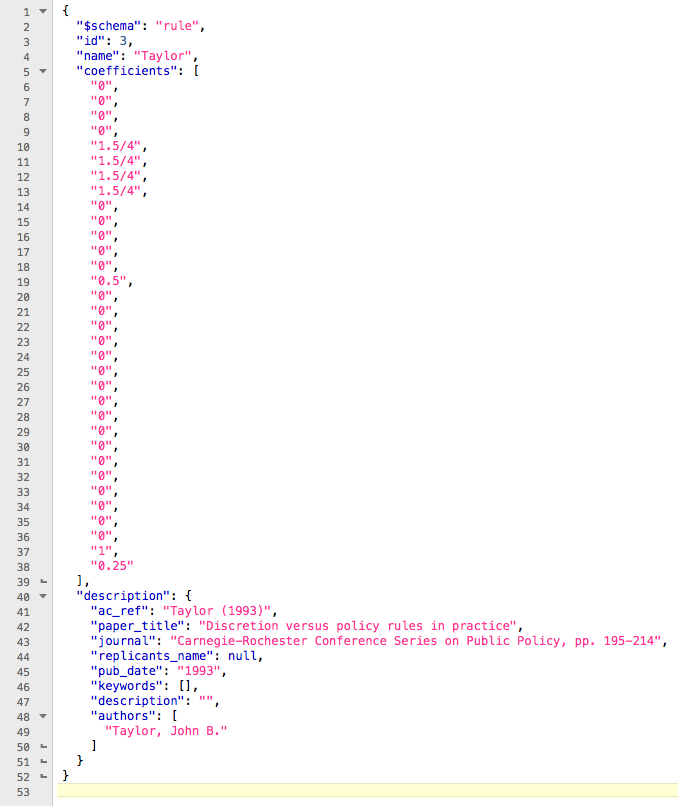
\includegraphics[width=13cm,keepaspectratio]{userrulejson.png}
        \label{img:userruletaylorjson}
        \end{figure}




\noindent {\it 1) Add a common monetary policy rule}\\
%\textbf{TO BE COMPLETED}
\begin{itemize}
%  \item The first task is to choose a suitable name for the new policy rule and to include it into an array for a list of rule names, \emph{rulenames}. One also has to add its acronyms in character arrays, \emph{rulenamesshort} and \emph{rulenamesshort1} \footnote{ As \emph{rulenamesshort1} are used for displaying simulation outcomes in Matlab console, any blank is not allowed in the rule name.}. Please make sure that the new rule name is of the same size of character array as the already existing one. Next, one assigns color to the rule with the array \textit{myrulecolor}.
%	\item Then, one adds the specification of the new-rule coefficients right after the last common rule's specification.
%  \item The remaining work is to add the new rule to the frontend of the MMB 3.0 \\\textbf{TO BE COMPLETED}.
\item In the new version of the MMB, policy rules are entirely defined via json-files. Common policy rules are stored in the subfolder `resources/app/dist/electron/static/mmci-cli/rules'.
\item The first task is to choose a suitable name for the new policy rule and to create a json-file with the same name. This json-file is to be stored in a subfolder with the exactly same name in the \textit{RULE} folder.
\item The json-file for a rule is in general similar to those for models; the whole entry has to be in curly brackets (\{...\}) and blocks are separated by commas. Figure \ref{img:userruletaylorjson} shows an exemplary json-file for the Taylor (1993) rule.
\item First, you have to indicate that the json-file describes a policy rule by setting \texttt{"\$schema": "rule"},
\item Second, you have to give the new rule an id-number by specifying \texttt{"id":\textit{number}}. The number 3 to 11 are already taken by the common policy rules shipped with the MMB.
\item Third, give your rule a name by specifying \texttt{"name": \textit{name}}, which should be the same you have given to the folder and the json-file.
\item Fourth, you have to actually specify the parameters of the rule by setting \texttt{"coefficients": $[$...$]$} to the respective values.
\item Fifth, you need to add a description of the rule, very much like you do in the json-files for models as described in section \ref{sec:ModelfileStructure}. Here, you can set \texttt{"replicants\_name": null}.
\item Safe the json-file and go to the MMB interface, click on `Menu' and `Reload Data'. The new rule should now be displayed under `Policy rules'
\item However, in order to use the new rule for comparison exercises, you also need to add its \texttt{id} to the \texttt{rules} section of all model-jsons for which the rule can/shall be used. This is necessary because not all models can be solved with all parameterizations (see subsection 3 of this chapter) and the new MMB is designed such that only common policy rules can be selected in combination with models in which they actually work. When you have done this, again reload data in the interface. The new rule should now be fully implemented in your MMB.


\end{itemize}


\noindent {\it 2) Add the model-specific monetary policy rule}

\begin{itemize}
  \item When adding a new model, it is possible to include its policy rule as long as the rule can be rewritten in terms of Modelbase common variables. If this is the case, the user should specify the parameters of the model-specific rule in the \texttt{"msr"} section of the model's json-file.
%  add the model identification number to the variable vector \emph{model\_with\_rule} in the  file \emph{MMB\_settings.m} such that a model-specific rule is activated when its corresponding model is chosen in \textbf{Option 2}. Otherwise, the user should add the model number to the variable vector \emph{model\_without\_rule}. For example, if the policy rule is set for the interest rate to react to exchange rate or credit growth, the user cannot include the original rule in the Modelbase.
%  \item Finally, the user has to insert the specification of the model-specific rule into the part of \emph{switch} statement in the file \emph{MMB\_OPTIONS/MSR\_COEFFFS.m} using the model's identification number as the case expression.
\item Reload data in the interface to employ the changes in the MMB.
\end{itemize}

\noindent {\it 3) User-specified monetary rule}

\begin{itemize}
  \item When \textit{User-specified rule} is chosen (see figure \ref{img:PR} in section \ref{sec:usingMMB}), a menu with a general form of a monetary policy rule appears in terms of common variables. Then, one can specify desired coefficient values of each variable in columns and to the corresponding lag/lead in rows.
      For example, to implement the Taylor (1993) rule using the option for user-specified monetary policy rule, one should set the coefficients as following: $ \rho_{\pi,0} = \rho_{\pi,-1} = \rho_{\pi,-2} = \rho_{\pi,-3} = 0.375, \rho_{q,0} = 0.5 $ and the rest of coefficients to zero. Figure \ref{img:userruletaylor} illustrates how to use the option for a user-specified rule with the example of Taylor (1993) rule. \\

        \begin{figure}[H]
        \centering
        \caption{\textsc{Taylor (1993) rule using the option of user-specified rule }}
        \vspace{0.2cm}
        \includegraphics[width=13cm,keepaspectratio]{userrule.png}
        \label{img:userruletaylor}
        \end{figure}

  \item Note that with certain rule parametrization, models cannot be solved due to several reasons. For example, the system of equations may violate the Blanchard-Kahn conditions so a model does not yield a unique stationary rational expectations equilibrium. There is no clear guideline for conditions for determinacy, but \cite{LevinWielandWilliams2003} suggest several crucial characteristics of rules that deliver a unique equilibrium: a relatively short inflation forecast horizon, a moderate degree of responsiveness to the inflation forecast, an explicit response to the current output gap, and a substantial degree of policy inertia.
\end{itemize}


There are three ways to add a new rule to the Modelbase: 1) add a rule to a list of common monetary policy rules, 2) include the model-specific rule calibrated or estimated by the original model authors and 3) specify a rule using the Modelbase user-specified rule option. Below we discuss each case in detail. Keep in mind that policy rules in the Modelbase have to be reformulated in terms of common Modelbase variables such as the annualized quarterly interest rate, the annualized quarter-to-quarter rate of inflation, the quarterly output and the quarterly output gap. This is explained in detail in \cite{WCMSW2012} and in the separate document, called 'MMB\_MPrule\_description.pdf'. 
%Also, one can see how it practically works by looking at common monetary policy rules already implemented in the \emph{MMB\_OPTIONS/MMB\_settings.m} file.
\newline


        \begin{figure}
        \centering
        \caption{\textsc{Taylor (1993) rule as defined in json-file}}
        \vspace{0.2cm}
        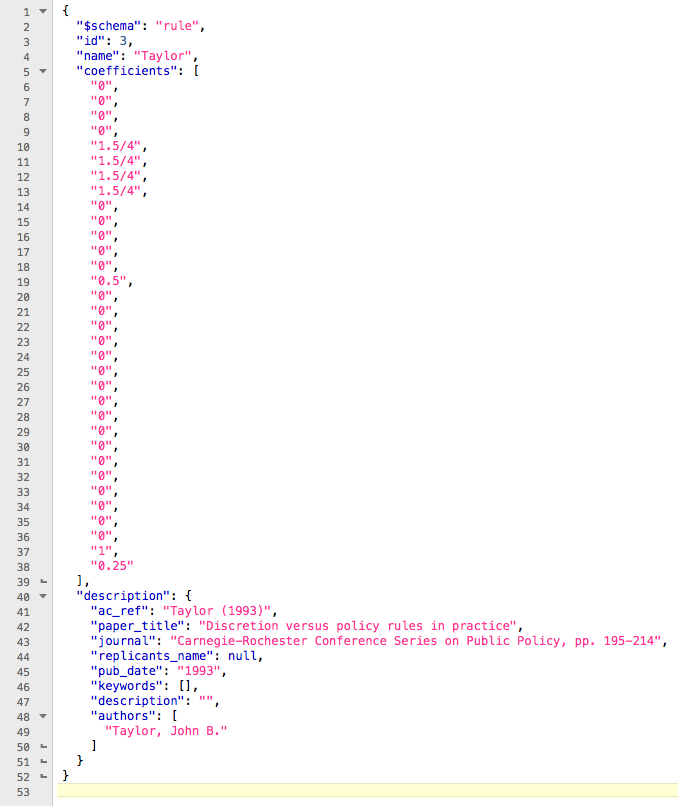
\includegraphics[width=13cm,keepaspectratio]{userrulejson.png}
        \label{img:userruletaylorjson}
        \end{figure}




\noindent {\it 1) Add a common monetary policy rule}\\
%\textbf{TO BE COMPLETED}
\begin{itemize}
%  \item The first task is to choose a suitable name for the new policy rule and to include it into an array for a list of rule names, \emph{rulenames}. One also has to add its acronyms in character arrays, \emph{rulenamesshort} and \emph{rulenamesshort1} \footnote{ As \emph{rulenamesshort1} are used for displaying simulation outcomes in Matlab console, any blank is not allowed in the rule name.}. Please make sure that the new rule name is of the same size of character array as the already existing one. Next, one assigns color to the rule with the array \textit{myrulecolor}.
%	\item Then, one adds the specification of the new-rule coefficients right after the last common rule's specification.
%  \item The remaining work is to add the new rule to the frontend of the MMB 3.0 \\\textbf{TO BE COMPLETED}.
\item In the new version of the MMB, policy rules are entirely defined via json-files. Common policy rules are stored in the subfolder `resources/app/dist/electron/static/mmci-cli/rules'.
\item The first task is to choose a suitable name for the new policy rule and to create a json-file with the same name. This json-file is to be stored in a subfolder with the exactly same name in the \textit{RULE} folder.
\item The json-file for a rule is in general similar to those for models; the whole entry has to be in curly brackets (\{...\}) and blocks are separated by commas. Figure \ref{img:userruletaylorjson} shows an exemplary json-file for the Taylor (1993) rule.
\item First, you have to indicate that the json-file describes a policy rule by setting \texttt{"\$schema": "rule"},
\item Second, you have to give the new rule an id-number by specifying \texttt{"id":\textit{number}}. The number 3 to 11 are already taken by the common policy rules shipped with the MMB.
\item Third, give your rule a name by specifying \texttt{"name": \textit{name}}, which should be the same you have given to the folder and the json-file.
\item Fourth, you have to actually specify the parameters of the rule by setting \texttt{"coefficients": $[$...$]$} to the respective values.
\item Fifth, you need to add a description of the rule, very much like you do in the json-files for models as described in section \ref{sec:ModelfileStructure}. Here, you can set \texttt{"replicants\_name": null}.
\item Safe the json-file and go to the MMB interface, click on `Menu' and `Reload Data'. The new rule should now be displayed under `Policy rules'
\item However, in order to use the new rule for comparison exercises, you also need to add its \texttt{id} to the \texttt{rules} section of all model-jsons for which the rule can/shall be used. This is necessary because not all models can be solved with all parameterizations (see subsection 3 of this chapter) and the new MMB is designed such that only common policy rules can be selected in combination with models in which they actually work. When you have done this, again reload data in the interface. The new rule should now be fully implemented in your MMB.


\end{itemize}


\noindent {\it 2) Add the model-specific monetary policy rule}

\begin{itemize}
  \item When adding a new model, it is possible to include its policy rule as long as the rule can be rewritten in terms of Modelbase common variables. If this is the case, the user should specify the parameters of the model-specific rule in the \texttt{"msr"} section of the model's json-file.
%  add the model identification number to the variable vector \emph{model\_with\_rule} in the  file \emph{MMB\_settings.m} such that a model-specific rule is activated when its corresponding model is chosen in \textbf{Option 2}. Otherwise, the user should add the model number to the variable vector \emph{model\_without\_rule}. For example, if the policy rule is set for the interest rate to react to exchange rate or credit growth, the user cannot include the original rule in the Modelbase.
%  \item Finally, the user has to insert the specification of the model-specific rule into the part of \emph{switch} statement in the file \emph{MMB\_OPTIONS/MSR\_COEFFFS.m} using the model's identification number as the case expression.
\item Reload data in the interface to employ the changes in the MMB.
\end{itemize}

\noindent {\it 3) User-specified monetary rule}

\begin{itemize}
  \item When \textit{User-specified rule} is chosen (see figure \ref{img:PR} in section \ref{sec:usingMMB}), a menu with a general form of a monetary policy rule appears in terms of common variables. Then, one can specify desired coefficient values of each variable in columns and to the corresponding lag/lead in rows.
      For example, to implement the Taylor (1993) rule using the option for user-specified monetary policy rule, one should set the coefficients as following: $ \rho_{\pi,0} = \rho_{\pi,-1} = \rho_{\pi,-2} = \rho_{\pi,-3} = 0.375, \rho_{q,0} = 0.5 $ and the rest of coefficients to zero. Figure \ref{img:userruletaylor} illustrates how to use the option for a user-specified rule with the example of Taylor (1993) rule. \\

        \begin{figure}[H]
        \centering
        \caption{\textsc{Taylor (1993) rule using the option of user-specified rule }}
        \vspace{0.2cm}
        \includegraphics[width=13cm,keepaspectratio]{userrule.png}
        \label{img:userruletaylor}
        \end{figure}

  \item Note that with certain rule parametrization, models cannot be solved due to several reasons. For example, the system of equations may violate the Blanchard-Kahn conditions so a model does not yield a unique stationary rational expectations equilibrium. There is no clear guideline for conditions for determinacy, but \cite{LevinWielandWilliams2003} suggest several crucial characteristics of rules that deliver a unique equilibrium: a relatively short inflation forecast horizon, a moderate degree of responsiveness to the inflation forecast, an explicit response to the current output gap, and a substantial degree of policy inertia.
\end{itemize}


There are three ways to add a new rule to the Modelbase: 1) add a rule to a list of common monetary policy rules, 2) include the model-specific rule calibrated or estimated by the original model authors and 3) specify a rule using the Modelbase user-specified rule option. Below we discuss each case in detail. Keep in mind that policy rules in the Modelbase have to be reformulated in terms of common Modelbase variables such as the annualized quarterly interest rate, the annualized quarter-to-quarter rate of inflation, the quarterly output and the quarterly output gap. This is explained in detail in \cite{WCMSW2012} and in the separate document, called 'MMB\_MPrule\_description.pdf'. 
%Also, one can see how it practically works by looking at common monetary policy rules already implemented in the \emph{MMB\_OPTIONS/MMB\_settings.m} file.
\newline


        \begin{figure}
        \centering
        \caption{\textsc{Taylor (1993) rule as defined in json-file}}
        \vspace{0.2cm}
        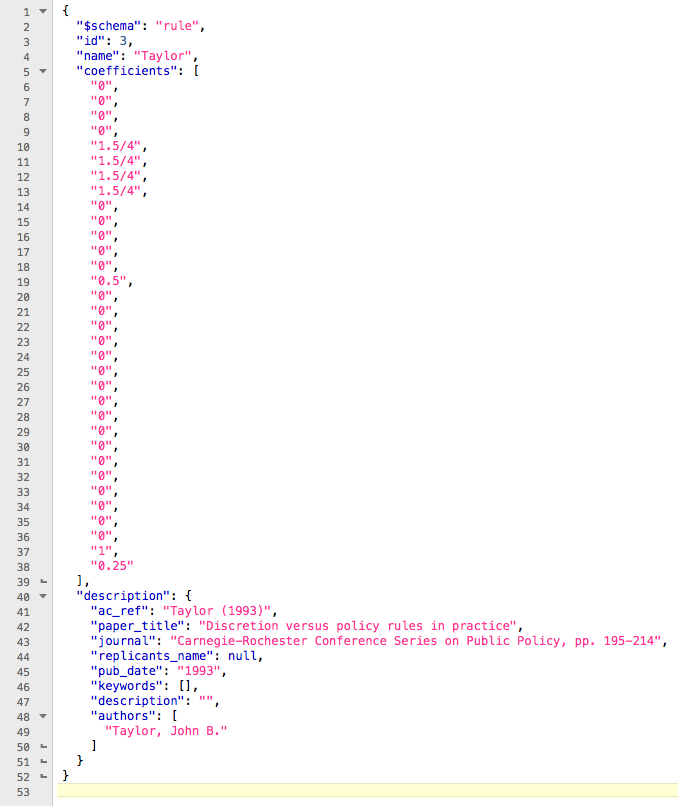
\includegraphics[width=13cm,keepaspectratio]{userrulejson.png}
        \label{img:userruletaylorjson}
        \end{figure}




\noindent {\it 1) Add a common monetary policy rule}\\
%\textbf{TO BE COMPLETED}
\begin{itemize}
%  \item The first task is to choose a suitable name for the new policy rule and to include it into an array for a list of rule names, \emph{rulenames}. One also has to add its acronyms in character arrays, \emph{rulenamesshort} and \emph{rulenamesshort1} \footnote{ As \emph{rulenamesshort1} are used for displaying simulation outcomes in Matlab console, any blank is not allowed in the rule name.}. Please make sure that the new rule name is of the same size of character array as the already existing one. Next, one assigns color to the rule with the array \textit{myrulecolor}.
%	\item Then, one adds the specification of the new-rule coefficients right after the last common rule's specification.
%  \item The remaining work is to add the new rule to the frontend of the MMB 3.0 \\\textbf{TO BE COMPLETED}.
%
%\item In the new version of the MMB, policy rules are entirely defined via json-files. Common policy rules are stored in the subfolder `resources/app/dist/electron/static/mmci-cli/rules'.
%\item The first task is to choose a suitable name for the new policy rule and to create a json-file with the same name. This json-file is to be stored in a subfolder with the exactly same name in the \textit{RULE} folder.
\item The policy rules that appear on the MMB interface are called “common” policy rules, which are saved as json-files in subfolders of `resources/app/dist/electron/static/mmci-cli/rules'. Adding your new policy rule as a common policy rule means that users need to create a json-file by following the steps below and save it in a subfolder of the same name in the same directory.
\item Please feel free to copy the format of any policy rule’s json-file provided in the MMB package to create your own json-file. While users should change some entries in the json-file based on their policy rules and preferences, please keep in mind that the style of punctuation marks should remain the same. 
In particular, the whole entry has to be in curly brackets (\{...\}) and blocks are separated by commas. Figure \ref{img:userruletaylorjson} shows an exemplary json-file for the Taylor (1993) rule.
%
%\item The json-file for a rule is in general similar to those for models; the whole entry has to be in curly brackets (\{...\}) and blocks are separated by commas. Figure \ref{img:userruletaylorjson} shows an exemplary json-file for the Taylor (1993) rule.
%\item First, you have to indicate that the json-file describes a policy rule by setting \texttt{"\$schema": "rule"},
\item For \texttt{"\$schema"}, keep \texttt{"rule"} as to indicate that the json-file describes a policy rule.
%\item Second, you have to give the new rule an id-number by specifying \texttt{"id":\textit{number}}. The number 3 to 11 are already taken by the common policy rules shipped with the MMB.
\item For \texttt{"id"}, assign any number other than 3 to 11, which are already taken for the existing common policy rule on the MMB.
%\item Third, give your rule a name by specifying \texttt{"name": \textit{name}}, which should be the same you have given to the folder and the json-file.
\item For \texttt{"name"}, type the name of the policy rule. It should be the same you have given to the json-file and the folder.
%\item Fourth, you have to actually specify the parameters of the rule by setting \texttt{"coefficients": $[$...$]$} to the respective values.
\item For \texttt{"coefficients"}, set the parameters of the policy rule. 
You have to specify 33 parameters.
	The first four entries describe the coefficients of lags 1 to 4 of the annualized quarterly nominal interest rate.
	Entries 5 to 13 are coefficients of the annualized quarterly inflation rate. It starts with current period inflation, followed by lags 1 to 4 of inflation and it ends with leads 1 to 4 of inflation. In case the inflation variable of the mod file is in quarterly frequency, the coefficient used there has to be annualized. Usually, it is multiplied by 4.
	Entries 14 to 22 belong to the output gap, while entries 23 to 31 belong to output. Both use the same structure as inflation. So the first is current period, followed by 4 entries for lags and 4 entries for leads.
	Entry 32 is the standard deviation of annual interest rate and entry 33 is the standard deviation of quarterly interest rate. It is a convention to set these values to "1" and "0.25" respectively.   
	In case a coefficient is not used in the policy rule, set it to "0".
%\item Fifth, you need to add a description of the rule, very much like you do in the json-files for models as described in section \ref{sec:ModelfileStructure}. Here, you can set \texttt{"replicants\_name": null}.
\item For \texttt{"description"}, change the entries based on the information of your new policy rule and type \texttt{null} for  \texttt{"replicants\_name"}.
%\item Safe the json-file and go to the MMB interface, click on `Menu' and `Reload Data'. The new rule should now be displayed under `Policy rules'
\item Save the json-file in the folder following the path specified in the first bullet point, i.e. `resources/app/dist/electron/static/mmci-cli/rules/NEWRULE/NEWRULE.json'. Click `Menu' and `Reload Data' on the MMB interface. Your new policy rule should appear in the list of `Policy Rules'.
%\item However, in order to use the new rule for comparison exercises, you also need to add its \texttt{id} to the \texttt{rules} section of all model-jsons for which the rule can/shall be used. This is necessary because not all models can be solved with all parameterizations (see subsection 3 of this chapter) and the new MMB is designed such that only common policy rules can be selected in combination with models in which they actually work. When you have done this, again reload data in the interface. The new rule should now be fully implemented in your MMB.
\item Users, however, need to manually add the new policy rule's id number in the jsons-files of models for which the new rule should be available for comparison exercises. To do so, add the id number in the section of \texttt{"rules"} under \texttt{"capabilities"}.

\end{itemize}


\noindent {\it 2) Add the model-specific monetary policy rule}

\begin{itemize}
%  \item When adding a new model, it is possible to include its policy rule as long as the rule can be rewritten in terms of Modelbase common variables. If this is the case, the user should specify the parameters of the model-specific rule in the \texttt{"msr"} section of the model's json-file.
\item Adding your new policy rule as a model-specific policy rule takes place when a new model is added and its policy rule can be re-written in terms of the MMB's common variables. Please specify the parameters of your new policy rule in the section of \texttt{“mrs”} in the json-file of your new model.
%  add the model identification number to the variable vector \emph{model\_with\_rule} in the  file \emph{MMB\_settings.m} such that a model-specific rule is activated when its corresponding model is chosen in \textbf{Option 2}. Otherwise, the user should add the model number to the variable vector \emph{model\_without\_rule}. For example, if the policy rule is set for the interest rate to react to exchange rate or credit growth, the user cannot include the original rule in the Modelbase.
%  \item Finally, the user has to insert the specification of the model-specific rule into the part of \emph{switch} statement in the file \emph{MMB\_OPTIONS/MSR\_COEFFFS.m} using the model's identification number as the case expression.
\item Click `Menu' and `Reload Data on the MMB interface. The new rule should now appear as `Model specific rule' in the list of `Policy Rules' when you select the new model.
\end{itemize}

\noindent {\it 3) User-specified monetary rule}

\begin{itemize}
%  \item When \textit{User-specified rule} is chosen (see figure \ref{img:PR} in section \ref{sec:usingMMB}), a menu with a general form of a monetary policy rule appears in terms of common variables. Then, one can specify desired coefficient values of each variable in columns and to the corresponding lag/lead in rows.
\item Adding your new policy rule as a user-specified policy rule takes place when `User-specified rule' is ticked on the MMB interface's `Policy Rules' list (see figure \ref{img:PR} in section \ref{sec:usingMMB}). Click `(edit)' and specify coefficients for the variables and time lags/leads.
\item For example, to implement the Taylor (1993) rule using the option for user-specified monetary policy rule, one should set the coefficients as following: $ \rho_{\pi,0} = \rho_{\pi,-1} = \rho_{\pi,-2} = \rho_{\pi,-3} = 0.375, \rho_{q,0} = 0.5 $ and the rest of coefficients to zero. Figure \ref{img:userruletaylor} illustrates how to use the option for a user-specified rule with the example of Taylor (1993) rule. \\

        \begin{figure}[H]
        \centering
        \caption{\textsc{Taylor (1993) rule using the option of user-specified rule }}
        \vspace{0.2cm}
        \includegraphics[width=13cm,keepaspectratio]{userrule.png}
        \label{img:userruletaylor}
        \end{figure}

  \item Note that with certain rule parametrization, models cannot be solved due to several reasons. For example, the system of equations may violate the Blanchard-Kahn conditions so a model does not yield a unique stationary rational expectations equilibrium. There is no clear guideline for conditions for determinacy, but \cite{LevinWielandWilliams2003} suggest several crucial characteristics of rules that deliver a unique equilibrium: a relatively short inflation forecast horizon, a moderate degree of responsiveness to the inflation forecast, an explicit response to the current output gap, and a substantial degree of policy inertia.
\end{itemize}

